\documentclass[a4paper]{ctexart}
\usepackage{geometry}
\usepackage{multicol}
\usepackage{pstricks}
\usepackage{graphics,graphicx}
\usepackage{pst-plot}
\usepackage{color}
\usepackage{amsmath}
\geometry{left=2cm,right=2cm,top=2.5cm,bottom=2.5cm}

\setCJKmainfont[BoldFont={SimHei},ItalicFont={KaiTi}]
  {FangSong}
\title{全书解答7}
\author{Chunwei Yan}
\date{\today}
\begin{document}
\maketitle
%---content here----
\begin{multicols}{2}

\section{极坐标详细讲解}
\par 极坐标和直角坐标一样,都是一种定位点的方式。

\subsection{定义}
\par 直角坐标系下,每个点由$(x,y)$定位,x,y分别是点按照x,y轴正方向离原点的距离
\par 极坐标由$(\theta,\rho)$决定,其中
\begin{enumerate}
  \item $\theta$表示角度,从轴逆时针旋转的角度
  \item $\rho$表示旋转的半径长度,就是点到原点的距离
\end{enumerate}
\par 极坐标下,每一个点就是这样由一个旋转角度$\theta$和一个半径长度$\rho$表示
\textcolor{blue}{Fiture 1}
\begin{center}
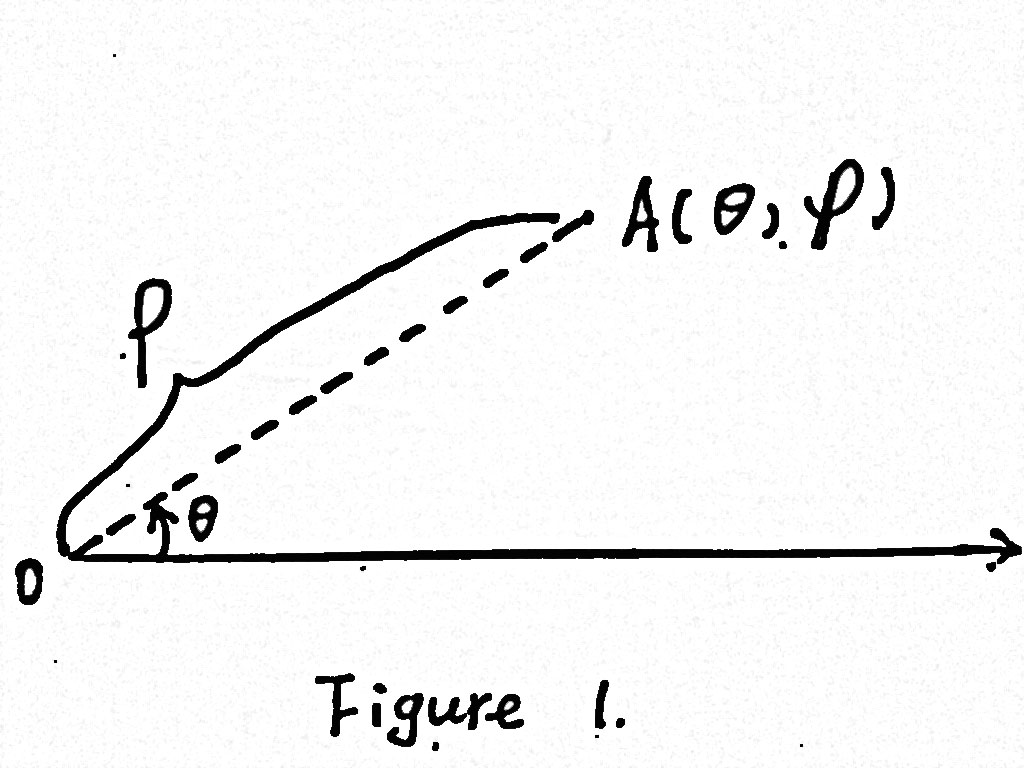
\includegraphics[height=5cm]{lecture7/Figure1.jpg}
\end{center}

\subsection{与直角坐标的转换}
\par 极坐标由角度$\theta$和旋转半径$\rho$决定,通过将计算,可以将相应的x,y算出来。

\textcolor{blue}{Fiture 2}
\begin{center}
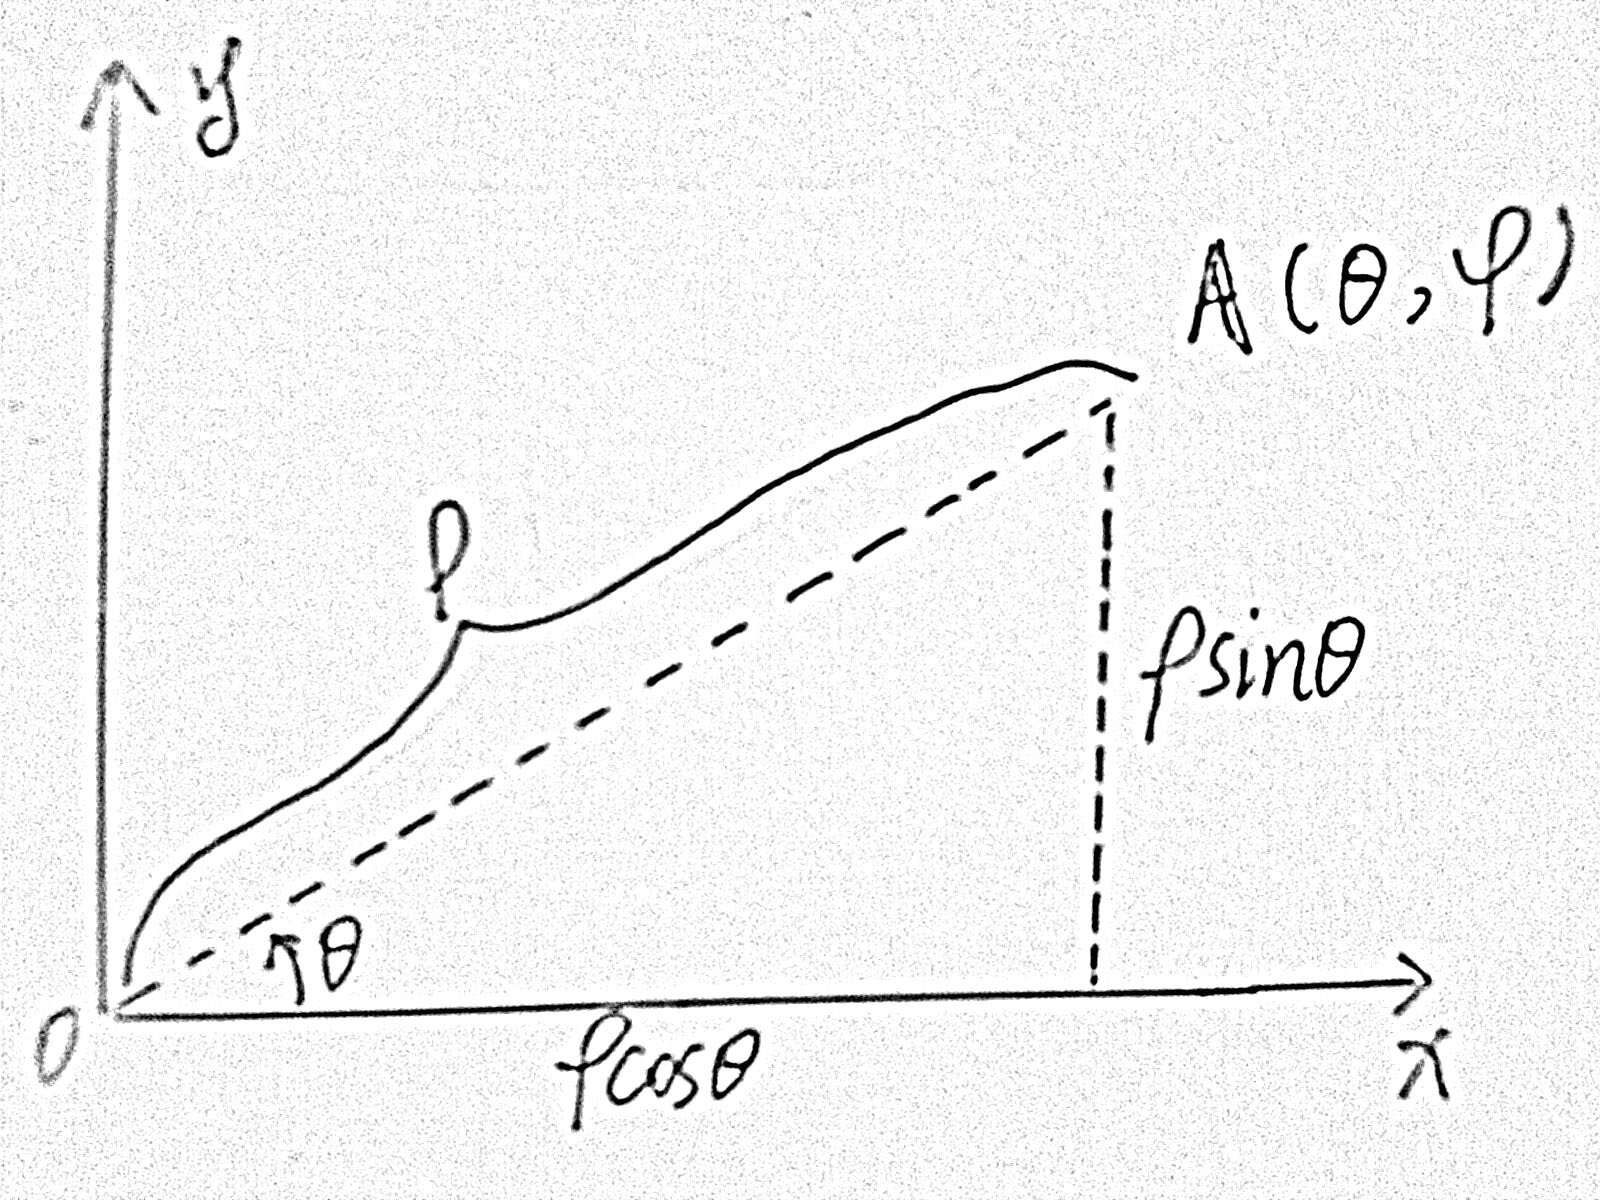
\includegraphics[height=5cm]{lecture7/Figure2.jpg}
\end{center}
\par 如图,横轴x的距离为$\rho\cos{\theta}$,纵轴y的距离为$\rho\sin{\theta}$,因此,其对应的直角坐标就是$(\rho\cos{\theta},\rho\sin{\theta})$

\subsubsection{简单的实例}
\begin{itemize}
  \item 极坐标到直角坐标:$(2, \frac{\pi}{6})\Rightarrow (\sqrt{3}, 1)$
  \item 直角坐标到极坐标:$(1,1) \Rightarrow (\frac{\sqrt{2}}{2}, \frac{\pi}{4})$
\end{itemize}

\subsection{二元函数的极坐标计算}
\subsubsection{二元函数积分的本质}
\par \textbf{参看全书P160}
\par 二元函数的积分公式里面包含两个部分:
\begin{equation}
\iint_{D}{f(x,y)d\sigma}
\end{equation}
\begin{enumerate}
    \item 积分区域$D$,用于规定积分的区域
    \item 积分函数$f(x,y)$,在积分区域内每个点计算和积分
\end{enumerate}
\textcolor{blue}{Fiture 2}
\begin{center}
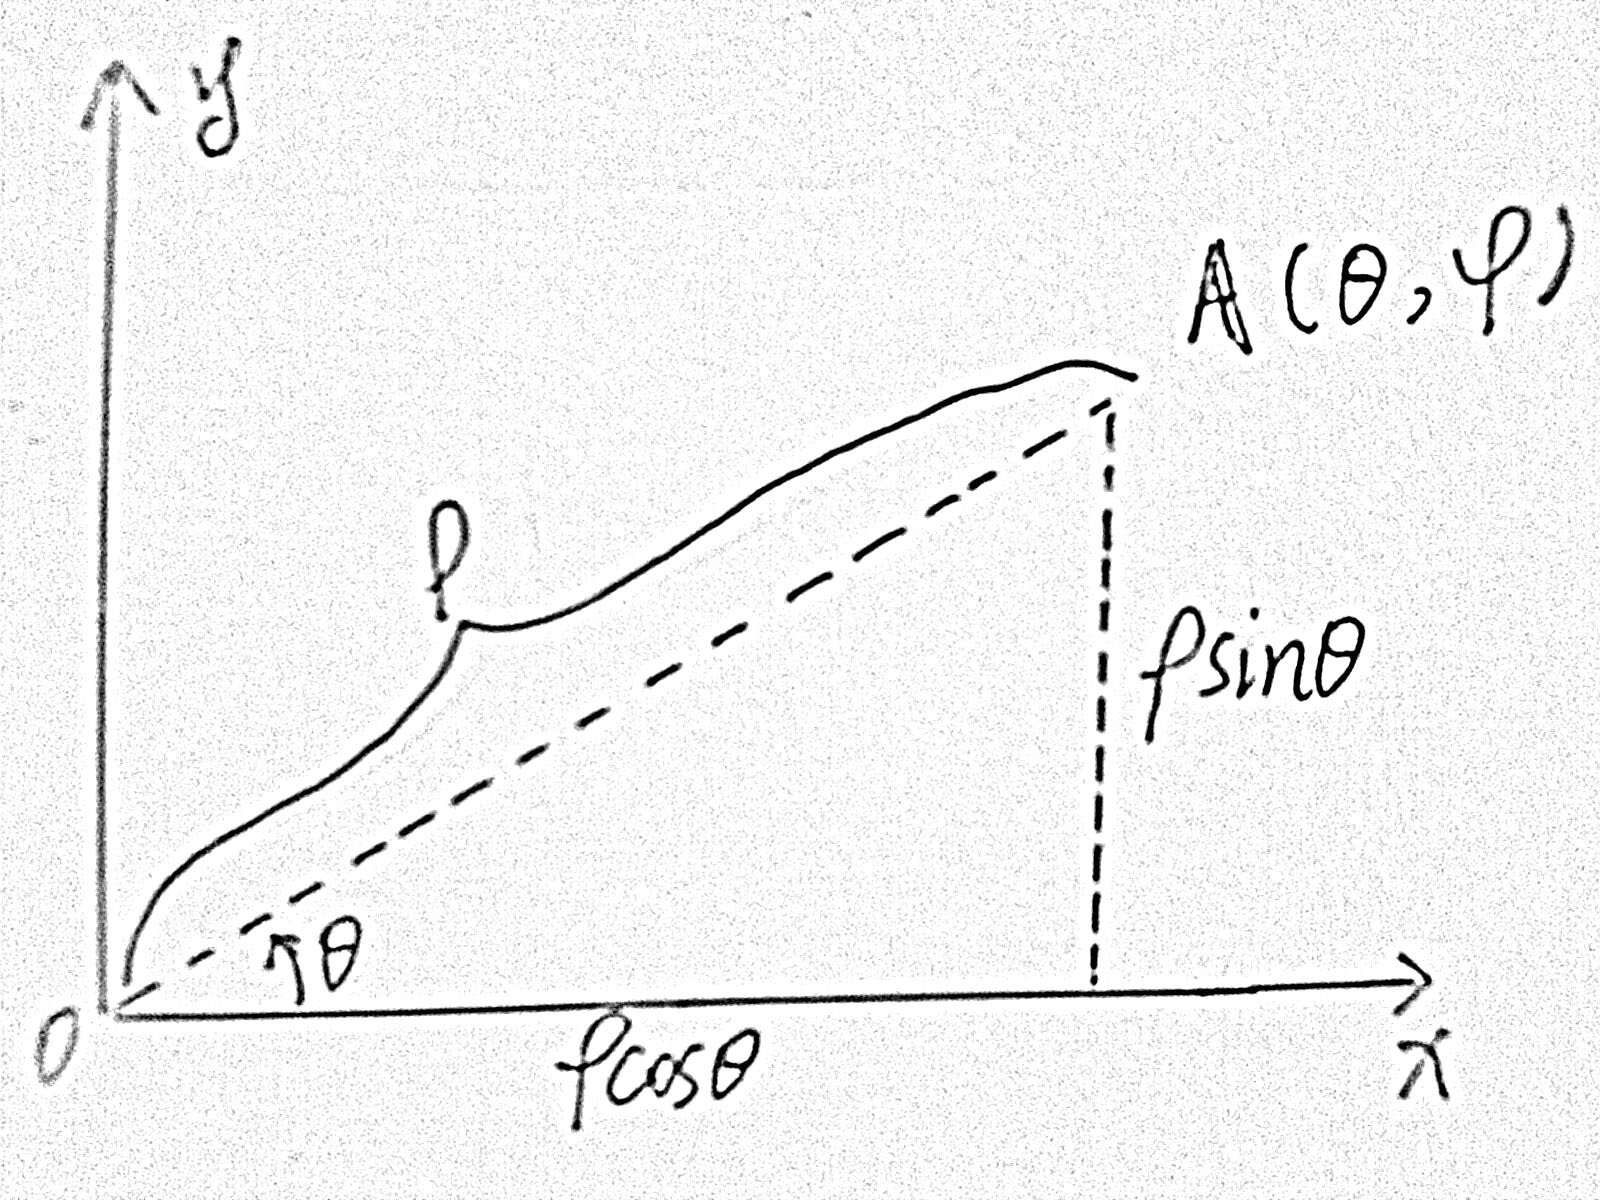
\includegraphics[height=5cm]{lecture7/Figure2.jpg}
\end{center}
\par 如图,阴影部分为积分区域
\par \textbf{积分区域规定积分函数积分的区域,除此之外,两者之间没有直接关系}

\subsubsection{用极坐标积分计算}
\par 用极坐标计算和用直角坐标计算原理是相通的,只需要将直角坐标系下的定义域$D$和积分函数$f(x,y)$用极坐标表示出来
其中,积分函数的转化比较简单,直接将$x,y$转换为$\rho\cos{\theta}, \rho{\sin{\theta}}$
\par 积分区域的转换
%--- img ---
\textcolor{blue}{Figure 4}
\begin{center}
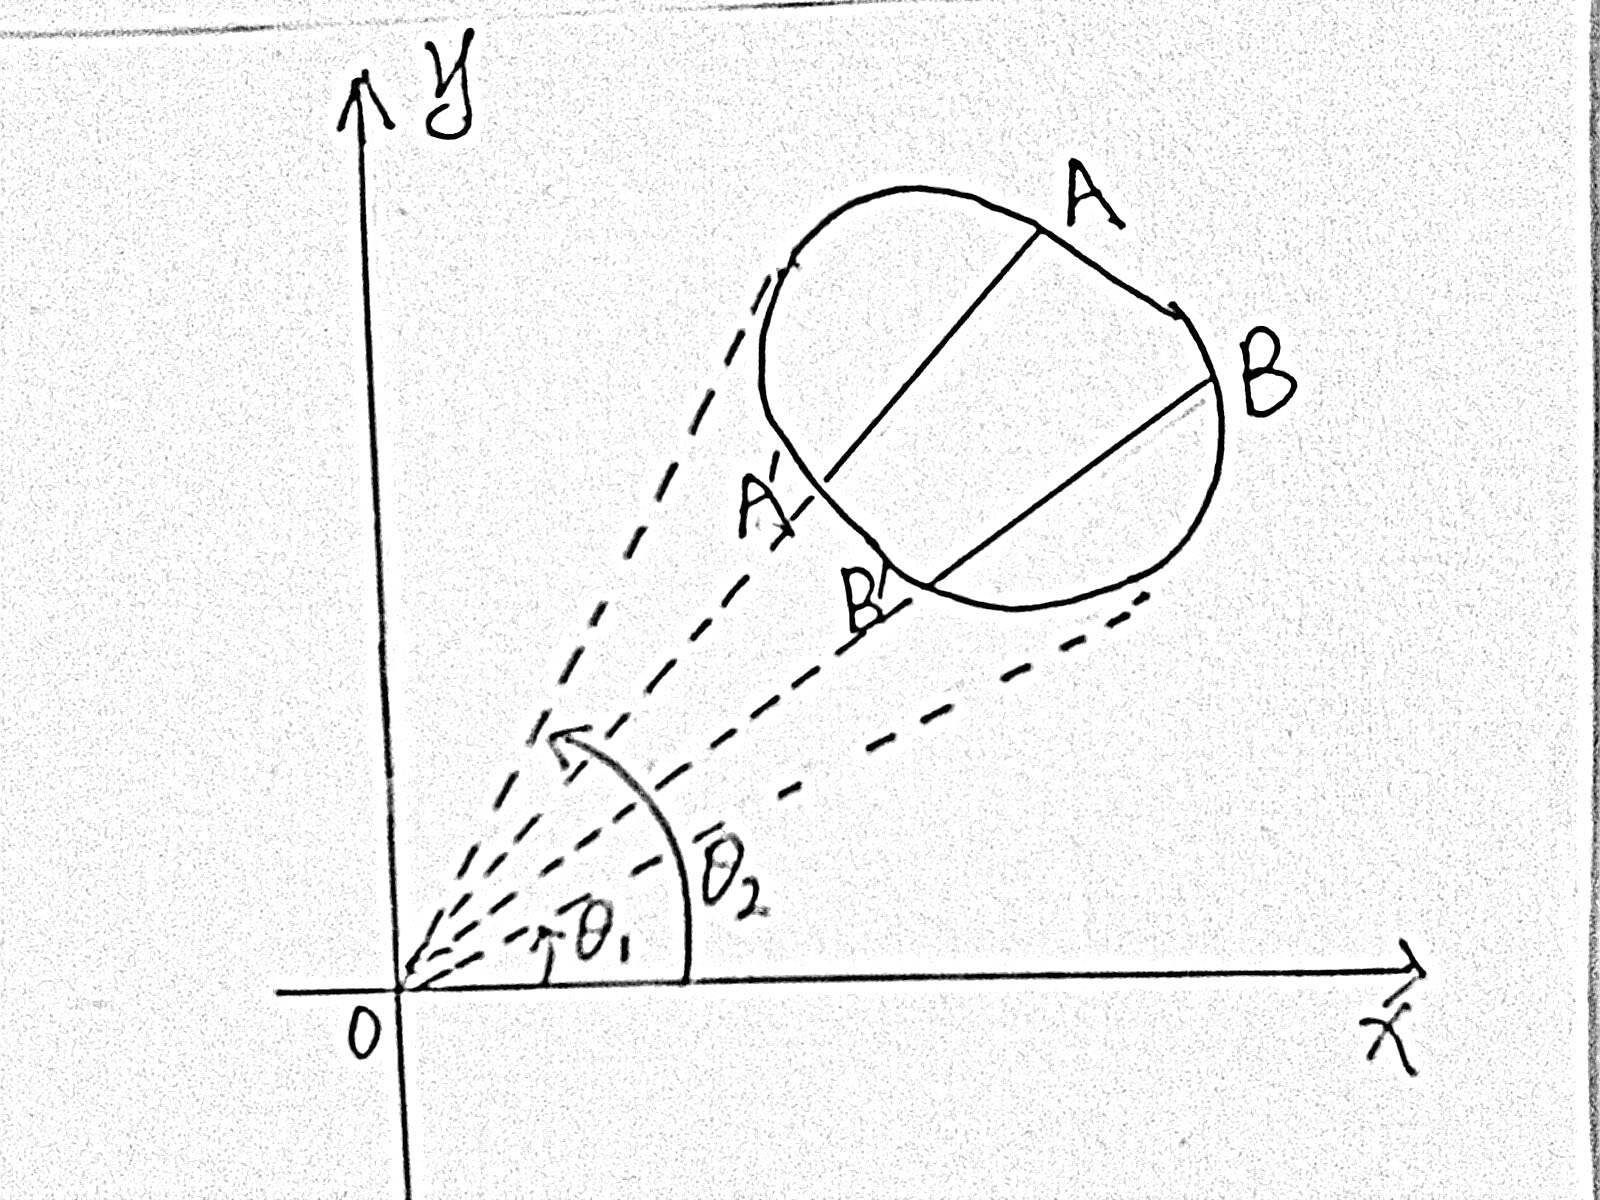
\includegraphics[height=5cm]{lecture7/Figure4.jpg}
\end{center}
%--- img ---
\par 见Figure 4
\par 极坐标下定义积分区域的方式:
\textbf{\textcolor{red}{注意,在极坐标下,只需要关心两点:旋转角度$\theta$. 旋转半径$\rho$}}
\par 可以想象,图中的积分区域是由一个线段沿着从$\theta_1$逆时针旋转到$\theta_2$画成的
\par 积分是无数个微观过程的总和,比如从角度$\theta_1$到$\theta_2$的过程中,其中两个线段: $AA'$和$BB'$,其中$AA' = \rho_A - \rho_A' = OA - OA'$
\par 如果无数个线段旋转着联合起来,就是下图
\textcolor{blue}{Figure 5}
\begin{center}
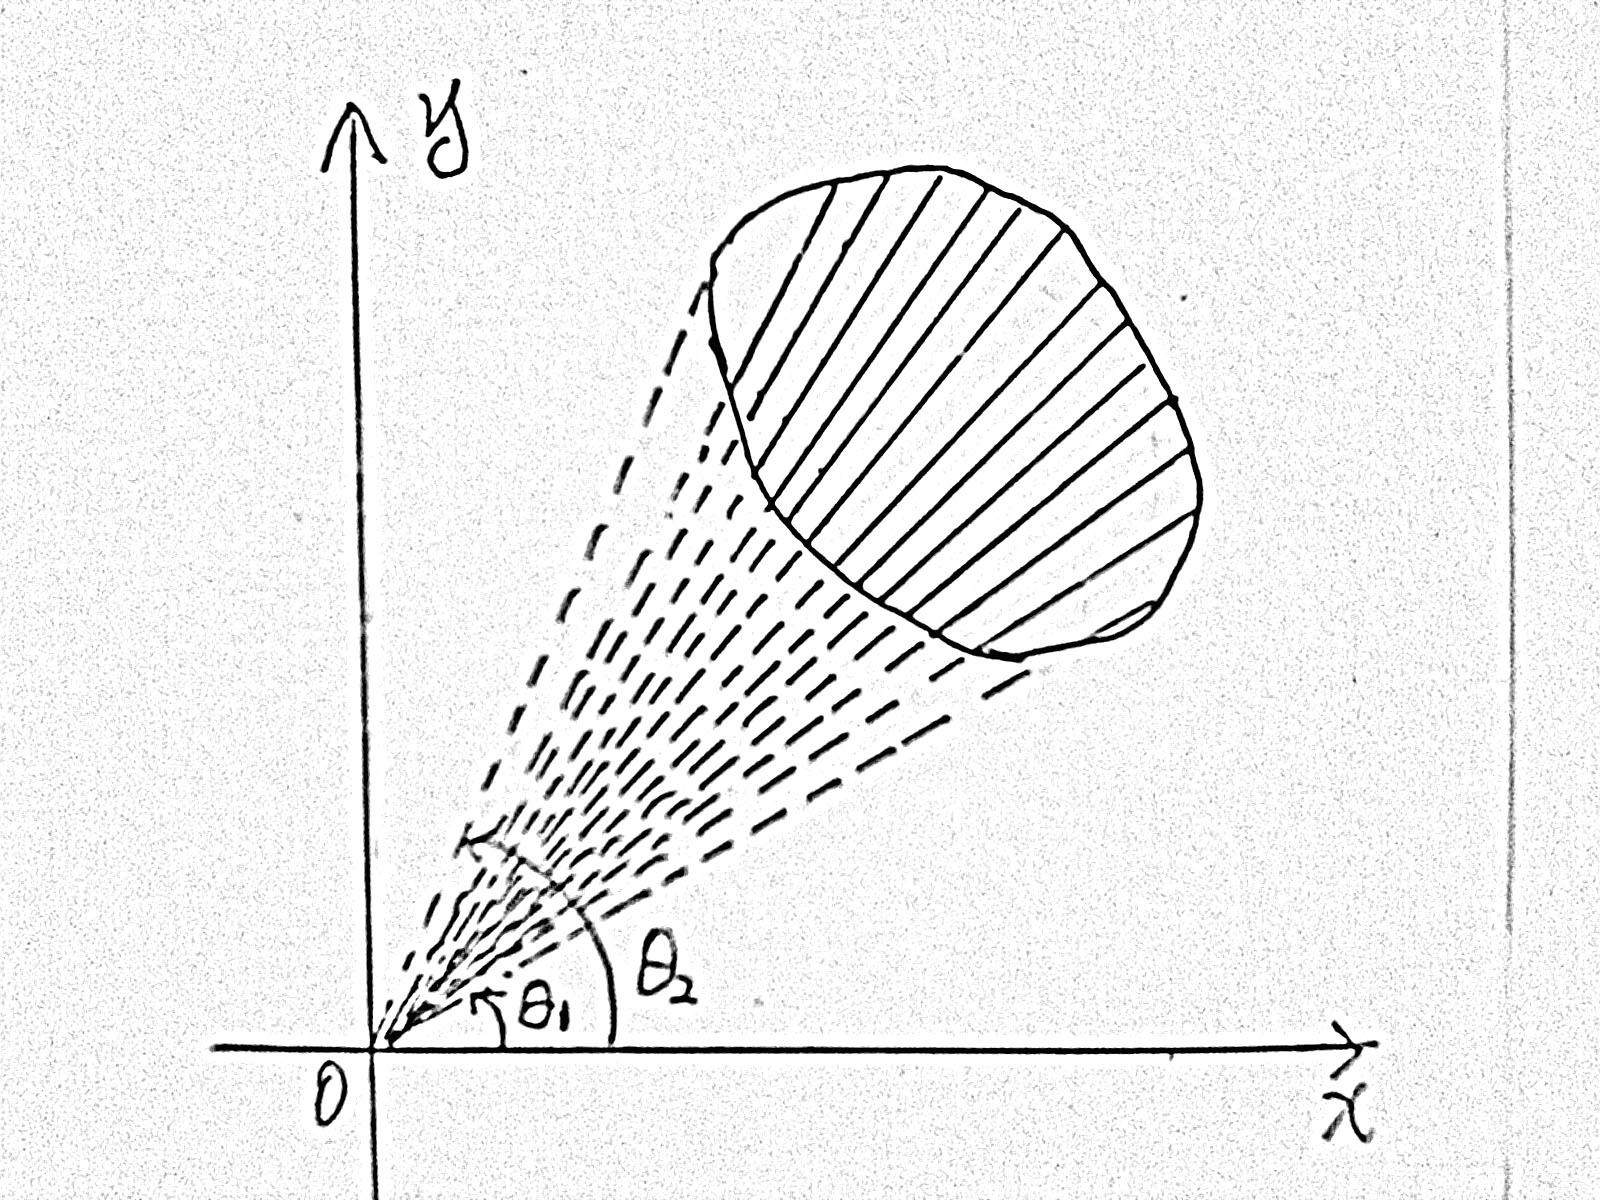
\includegraphics[height=5cm]{lecture7/Figure5.jpg}
\end{center}
\par 构成了一个积分区域,就是图中的阴影部分

\subsection{理解P160的几个公式}
\par 在全书P160(2)在极坐标下的计算中,列出了4个图,相应的有四种情况

\subsubsection{极点O在区域D之外}
%--- img ---
\textcolor{blue}{Figure 6}
\begin{center}
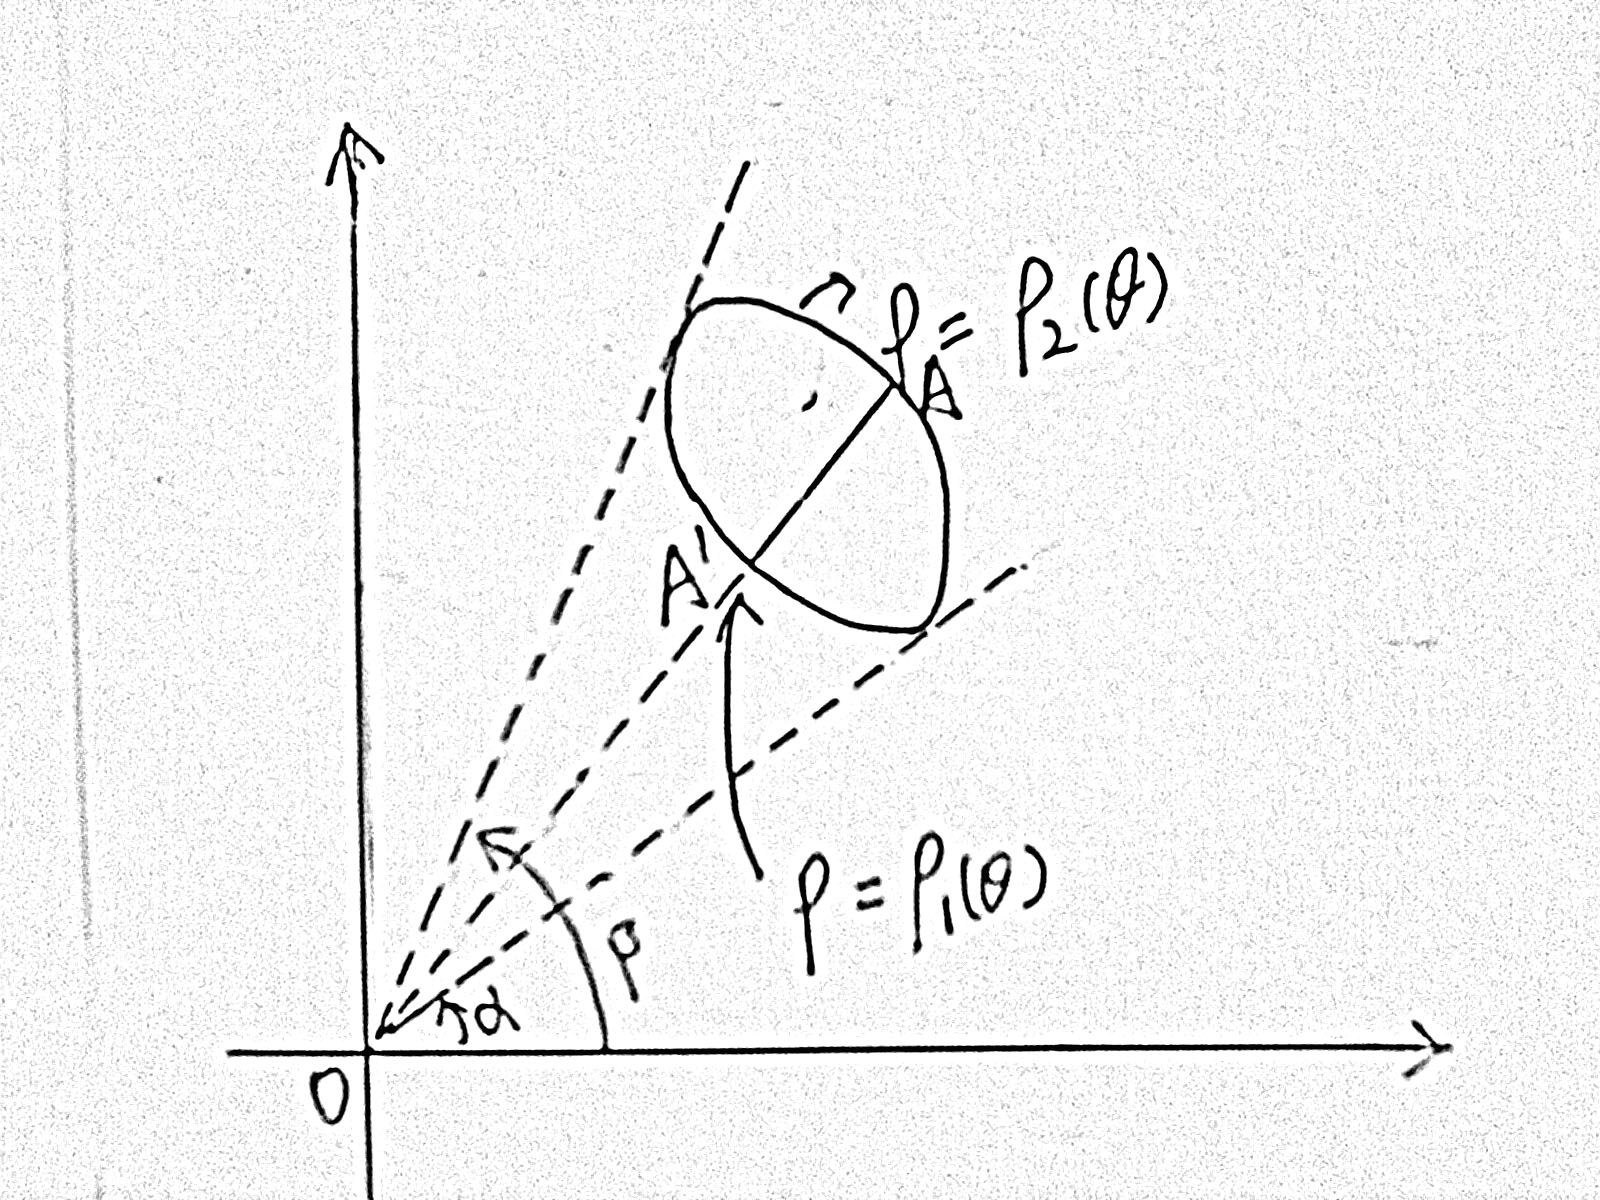
\includegraphics[height=5cm]{lecture7/Figure6.jpg}
\end{center}
%--- img ---
\par 看Figure 6
\par 联合之前讲的例子,AA'是构成极坐标下积分域中的一条线段,如果设$\theta_A$是A对应的角度
\par 很明显
\begin{equation}
AA' = \rho_2(\theta_A) - \rho_1(\theta_A)
\end{equation}
\par 首先,当然积分函数$f(\rho\cos{\theta}, \rho\sin{\theta})$最容易确定(x,y换成极坐标就可以了)
\par 然后定极坐标:
\begin{enumerate}
    \item 角度$\theta$,那么从$\alpha$逆时针旋转到$\beta$,于是有$\int_{\alpha}^{\beta}$
    \item (线段构成的)轮廓 从图中看,之前讲过,无数条绕着O旋转的线段构成了积分域(阴影部分),其中AA'只是其中的一条
    \par 对于这当中的任何一个角度$\theta$的线段,长度为 $L = \rho_2(\theta) - \rho_1(\theta)$
    \par 于是有了
    \begin{equation}
        \int_{\alpha}^{\beta}\int_{\rho_1(\theta)}^{\rho_2(\theta)}
    \end{equation}
\end{enumerate}

\par 添上极坐标下的积分函数,再加上固定项$\rho d \rho$,\textcolor{red}{\textbf{这个注意,只要是极坐标下的二元积分,都是这个固定项$\rho d \rho$,而不是$d\rho$}}
\par 最后就是
\begin{equation}
\iint_{D}{f(x,y)d\sigma} = \int_{\alpha}^{\beta}{d\theta}\int_{\rho_1(\theta)}^{\rho_2(\theta)}{f(\rho\cos{\theta}, \rho\sin{\theta})\rho d\rho}
\end{equation}
\par 参照上面的式子,可以理解为
\begin{itemize}
\item 角度$\theta$从$\alpha$积分到$\beta$,旋转的总角度为$\beta - \alpha$
\item 对应着每一个角度$\theta$ ,在射线方向上从$\rho_1(\theta)$积分到$\rho_2(\theta)$,对应的线段长度为$\rho_2(\theta) - \rho_1(\theta)$
\end{itemize}
\subsubsection{极点O在区域D的边界上}
%--- img ---
\textcolor{blue}{Figure 7}
\begin{center}
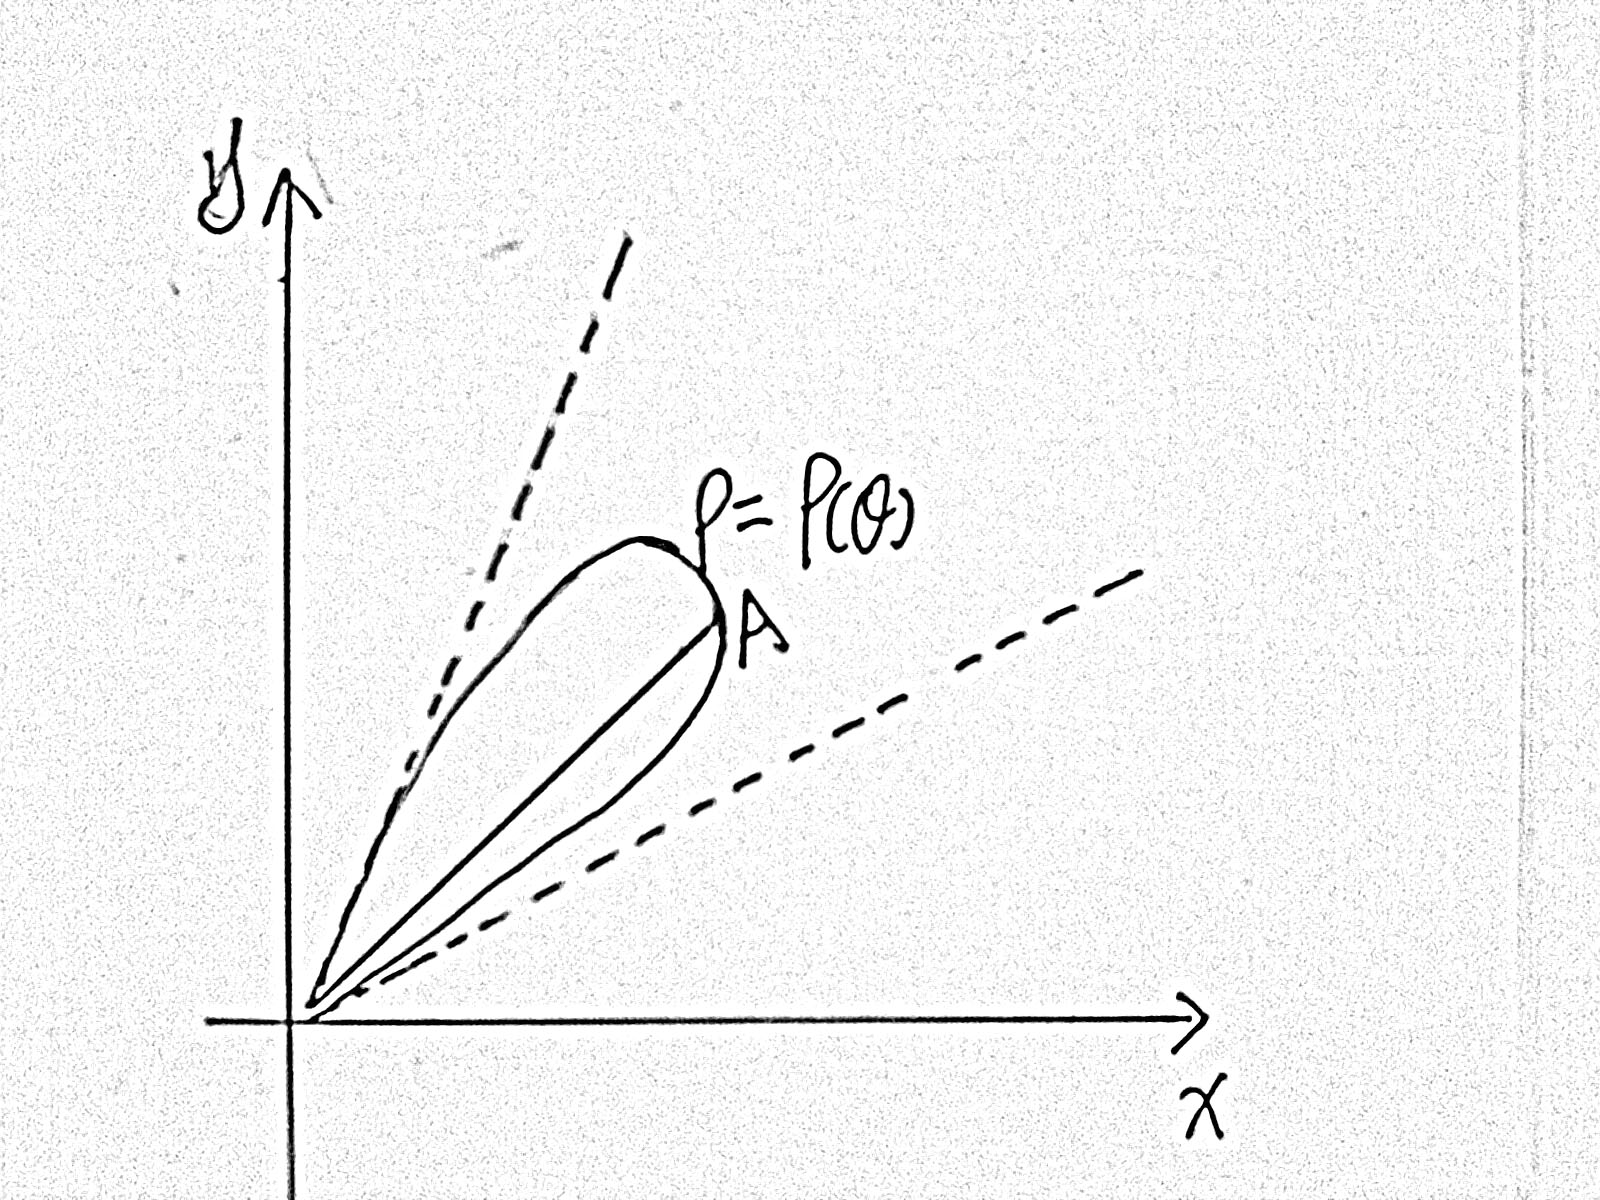
\includegraphics[height=5cm]{lecture7/Figure7.jpg}
\end{center}
%--- img ---
\par 角度$\theta$的情况与上面一个图没有变化,只是轮廓发生了变化
\par 如图,每一个旋转的线段,总有一个端点在原点,于是,线段的长度就是
\begin{equation}
OA = \rho(\theta) - 0
\end{equation}
\par 类比于上一个情况,其积分成为
\begin{equation}
\iint_{D}{f(x,y)d\sigma} = \int_{\alpha}^{\beta}{d\theta}\int_{0}^{\rho(\theta)}{f(\rho\cos{\theta}, \rho\sin{\theta})\rho d\rho}
\end{equation}

\subsubsection{极点O在区域D的内部}
\par 这个很直观,就是角度需要旋转一周$2\pi$,然后每一条旋转的线段类似于上面一种情况,从0到$\rho(\theta)$

\subsubsection{O在环形域内部}
\par 角度旋转一周($2\pi$),然后积分域中每一条旋转的线段类似于上面一种情况,从0到$\rho(\theta)$

\section{P173例65}
\par 现在应该能够直观看出极坐标了,旋转角度$\theta$是0到$2\pi$
\par 轮廓的话,就是将
\begin{equation}
\begin{cases}
\begin{array}{l}    
x = \rho \cos{\theta} \\
y = \rho \sin{\theta}
\end{array}    
\end{cases}
\end{equation}
代入就可以了。

\section{P173例66}
\par 倒数第二行积分的计算
\par 首先$\int{8\pi tdt} = 4\pi t^2$
\par 然后,在方括号里面
\begin{equation}
\int{8\pi t e^{4\pi t^2} e^{-\int{8\pi tdt}}dt} + C
\end{equation}
\par 好好分析形式,不要被吓着
\par 上面已经得到了$\int{8\pi tdt} = 4\pi t^2$,代进去
\begin{equation}
\int{8\pi t e^{4\pi t^2} e^{-\int{8\pi tdt}}dt + C}
= \int{8\pi t e^{4\pi t^2} e^{-4\pi t^2}dt + C}
\end{equation}
\begin{equation}
=
\int{8\pi tdt + C}
= 4\pi t^2 + C
\end{equation}
\par 如此,就算出来了。注意积分号的范围就行了.

\section{P174例67}

\subsection{积分中值定理}

\subsubsection{一元函数}
\par 如果$f(x)$在积分范围内连续
\begin{equation}
\ni \eta \in (a,b) s.t. \int_{a}^{b}{f(x)dx} = (b-a)f(\eta)
\end{equation}
\par 用线段ab中的一点$\eta$的值来作为线段中所有点的平均值
\par 平均值$f(\eta)$乘以线段长度(b-a)作为积分值

\subsubsection{二元函数}
\par 如果$f(x,y)$在积分范围内连续
\begin{equation}
\ni \alpha , \beta \in D s.t. \iint_{D}{f(x,y)d\sigma}
= S(D)f(\alpha, \beta)
\end{equation}
\par 用积分域D中的一点$(\alpha,\beta)$来作为D中所有点的平均值
\par 平均值$f(\alpha, \beta)$乘以积分域的面积$S(D)$作为积分值

\subsubsection{极限中采用积分中值定理}
\par 如果积分区域中有自变量有极限
\par 如一元函数中,有$\lim_{x\rightarrow 0}{\int_{0}^{x}{f(t)dt}}$
\par 当采用中值定理时,有$x\rightarrow 0, \eta \in (0, x)$ ,因此,$\eta \rightarrow 0$
\par 二元函数也类似
\subsection{方法一}
\par 从方法一第二行开始解释
\par 还是之前等价无穷小的知识点,回头回顾一下
\begin{equation}
f(x)\rightarrow 0; 1-e^{f(x)} \sim f(x) 
\end{equation}
\par 看到变限积分,而且上下都有x,就用对x求导的方式去掉一层积分号
\par 分子部分对x求导,去掉外层积分号,后面的u统一用x代替
\par 于是有
\begin{equation}
   -\lim_{x \rightarrow 0^+}
   {
       \frac{
           \int_{0}^{x^2}{f(t,x)dt}
       }
       {3x^2}
   } 
\end{equation}
\par x有一个极限,下面采用积分中值定理


\par 题目中方法一倒数第三行
\begin{equation}
-\lim_{x \rightarrow 0+}{
    \frac{
        \int_{0}^{x^2}{f(t,x)dt}
    }
    {3x^2}
}
\end{equation}
\par 首先,分子是对t求导,这个要注意,不是对x求导,因此,积分号里面x可以当作为一个常量,对实际的积分运算没有一点关系
\par 采用中值定理,分子部分变成
\begin{equation}
\ni c \in (0, x^2) s.t. \int_{0}^{x^2}{f(t,x)dt}
= x^2f(c,x)
\end{equation}
\par 这里因为$x\rightarrow 0$,而$c \in (0, x^2)$夹在其中,于是$c\rightarrow 0$
\par 于是有
\begin{equation}
\lim_{x\rightarrow 0^+, c\in(0, x^2)}{f(c,x)} = f(0,0)
\end{equation}

\subsection{方法二}
\par 直接采用了积分中值定理,而且利用了夹逼性得到其极限
\par 看P175上面第一个式子的分母
\begin{equation}
\int_{0}^{x^2}dt\int_{x}^{\sqrt{t}}{f(t,u)du}
=
f(\xi, \eta) \cdot \frac{1}{3}x^3
\end{equation}
\par 其中$\frac{1}{3}x^3$是积分域D的面积,$(\xi, \eta) \in D$
因为$x\rightarrow 0^+$,因此使得整个D趋近于0,因此$f(\xi,\eta) \rightarrow 0$

















\end{multicols}
\end{document}
